\documentclass{elteikthesis}


\usepackage{t1enc}
\usepackage{ucs}
\usepackage[utf8x]{inputenc}
\usepackage[T1]{fontenc}
\usepackage[english,hungarian]{babel}
\selectlanguage{hungarian}

\usepackage{listings}
\usepackage{color}
\usepackage{verbatim}


\definecolor{mygray}{rgb}{0.4,0.4,0.4}
\definecolor{mygreen}{rgb}{0,0.8,0.6}
\definecolor{myorange}{rgb}{1.0,0.4,0}

\lstset {
	basicstyle=\footnotesize\sffamily\color{black},
	commentstyle=\color{mygray},
	frame=single,
	%%numbers=left,
	%%numbersep=5pt,
	%%numberstyle=\tiny\color{mygray},
	keywordstyle=\color{mygreen},
	showspaces=false,
	showstringspaces=false,
	stringstyle=\color{myorange},
	tabsize=2
}

\title{Interpoláció osztott rendszereken}
\author{Cselyuszka Alexandra}
\supervisor{Tejfel Máté}
\supervisorstitle{egyetemi tanár}
\period{Informatika Bsc}
\thesisyear{2015}
\department{Programozási Nyelvek és Fordítóprogramok Tanszék}
%%\additionaltext{ABCDEF GHIJKLM NOPQRSTUV WXYZ}

\begin{document}

\frontmatter

	\maketitle

\mainmatter

\tableofcontents
	
\chapter{Bevezetés} 

\textit{
"A gyakorlatban soksor felmerül olyan probléma, hogy egy nagyon költségesen kiszámítható függvénnyel kellene egy megadott intervallumon dolgoznunk. Ekkor például azt tehetjük, hogy néhány pontban kiszámítjuk a függvény értékét, majd keresünk olyan egyszerűbben számítható függvényt, amelyik illeszkedik az adott pontokra." 	}
\cite{numanalbev}
\newline
\newline
A szakdolgozatom célja ezekre a problémákra megoldást adni elosztott környezetben. 
\section{Feladat elemzése}
Adott ponthalmazokból kívánunk egy közelítő polinómot becsülni. Ezeket különböző interpolációs technikával meg tudjuk adni, ki tudjuk számolni. Több interpolációs technika létezik, melyekből könnyen meg tudunk adni akár több polinómot is egy adott ponthalmazhoz.\newline
Ezekkel a számításokkal előfordulhat, hogy lassan futnak, főleg ha több inteprolációt kívánunk egyszerre számolni.
Ebben az esetben optimálisabb több gépen számolni a különböző ponthalmazokat.
\newline\newline
Ebben a feladatban egy speciális megvalósítása lesz ennek a számításnak. \newline
A grafikus része egy weboldal, melyen szerkeszthetjük a ponthalmazokat. A számítás részét egy szerver végzi amely figyeli a felcsatlakozó gépeket. Amikor kap egy számítandó adathalmazt, akkor több gép segítségével kiszámítja az eredményt. Ha minden részfeladat végzett, akkor vissza küldi a weboldalra, ahol az eredmények megtekinthetőek grafikus formában.
\newline\newline
\section{Feladat megvalósítása}
A \textbf{grafikus felület}  egy weboldal, mely javascript-ben és HTML-ben van megvalósítva.
 A felületen egy listát tekinthetünk meg, ahova több ponthalmazt is felvehetünk. \newline  Mentés hatásásra az értékek a háttérben eltárolódnak. A ponthalmazok közül választhatunk egyet, amely betölődik felületre.\newline A szerkesztő felület egy táblázatból és egy grafikonból áll, emellett még a különböző speciális számításra vonatkozó tulajdonságok (interpoláció típusa) valamint a grafikonon való megjelenítéshez tartozó tulajdonságok (polinóm pontosság, megtekintendő intervallum) is szerkeszthetőek. \newline Ha befejeztük a halmazok szerkesztését elküldhetjük a számítani kívánt értékeket a szerver felé.
\newline\newline
A \textbf{szerver} feladata hogy figyelje a felületről érkező adatokat. Ha az adathalmaz megérkezett, akkor a szerver kibontja az adatokat egy JSON-ból, és elindítja az elosztást. \newline
Az elosztáshoz a szerveren el kell indítani egy figyelő folyamatot amelyre lehetősége van egy külső gépnek felcsatlakozni. Amikor a szerveren indul egy számolás a felcsatlakozott gépeket lekérdezi, majd a feladatokat szétosztja.\newline
A szerver megvalósítása és a gépekre való szétosztás Erlang-ban lett megvalósítva. A JSON feldolgozásához Mochi-JSON lett alkalmazva. A feldolgozás után az adathalmazon végig megyünk és azok alapján felparaméterezzük, és meghívjuk a számítást végző függvényt.\newline
A számításhoz használt maximális gépek száma paraméterként megadható, de a tényleges számítást csak annyi gépen tujduk maximálisan végezni ahány gép felcsatlakozott a számításhoz.
\newline\newline
A \textbf{számítás} megvalósítása C++ nyelven történt. A paraméterek alapján a Lagrange-féle, Newtone-féle, Hermite-féle interpolációs technikák közül eldönti melyik esetet használja.\newline 
Valamint inverz interpolációt is választhatnak a Lagrange vagy a Newton interpoláció esetén. \newline
A programban implementálásra került egy egyszerű polinóm szorzás és össze adás, valamint az inteprolációkhoz szükséges függvények. Lagrange számítás a polinóm műveletek és a képlet felhasználásával valósult meg. Newton és Hermite esetén a kapott adatokból először a kezdő mátrixot kell legenerálni, majd kiszámítani. \newline
Abban az esetben ha Newton vagy Lagrange polinómot számolunk nem vesszük figyelembe a derivált pontokat, viszont figyelmbe vesszük ha inverz számítást kívánunk végezni. 


\chapter{Felhasználói dokumentáció}
\begin{comment}
A Felhasználói dokumentáció tartalmazza
- a megoldott probléma rövid megfogalmazását,
- a felhasznált módszerek rövid leírását,
- a program használatához szükséges összes információt

Magába foglalja a telepítési- (vagy üzemeltetési-) és a végfelhasználói leírást. Ezek
meghatározott célközönséghez szólnak, könnyen és gyorsan kell, hogy eligazítsák a
felhasználót a program használatában!

\end{comment}

\section{Bevezetés}
%% A feladat rövid ismertetése (mire való a szoftver)
%% Célközönség (kik, mikor, mire használhatják a programot)
\section{Telepítési utmutató}
\subsection{Rendszer követelmények}
%% A rendszer használatához szükséges minimális, illetve optimális HW/SW környezet
\subsection{Segédprogramok telepítése}
%% Első üzembe helyezés leírása – ha van ilyen –, a program indítása (kivéve, ha nem egy
%%önálló alkalmazásról, hanem egy meglévő rendszer új komponenséről van szó). Itt
%%ellenőrizzük, hogy a telepítési útmutató megfelel-e a valóságos telepítési folyamatnak.
\subsection{Szerver és segédgépek üzembe helyezése}
\subsection{Használati útmutató}
\subsubsection{Weboldal}
\subsubsection{Szerver}
%% Általános felhasználói tájékoztató (például a szokásostól eltérő képernyő-, billentyű-,
%%illetve egérkezelés leírása, teendők hibaüzenetek esetén stb.).
%% A rendszer funkcióinak ismertetése. A feladat jellegéből fakadóan célszerű lehet ezt
%%folyamatszerűen, képernyőképekkel alátámasztva bemutatni. A funkciókat ajánlatos a
%%felhasználói szintek szerint csoportosítani. Itt vegyük figyelembe, hogy a leírás a
%%fejlesztői dokumentációban meghatározott részfeladathoz illeszkedik-e, az ott
%% meghatározott funkciókat/használati eseteket írja-e le?
%% A rendszer futás közbeni üzenetei (hibaüzenetek, figyelmeztető üzenetek, felszólító üze-
%%netek stb.) és azok magyarázata – az esetleges üzemeltetési teendőkkel együtt. Itt vegyük
%%figyelembe, hogy tartalmaz-e biztonsági, illetve hibaelhárítási előírásokat?
%% Egyéb, a szoftver használatához szükséges információk.

\chapter{Fejlesztői dokumentáció}
\begin{comment}
A Fejlesztői dokumentáció tartalmazza
- a probléma részletes specifikációját,
- a felhasznált módszerek részletes leírását, a használt fogalmak definícióját,
- a program logikai és fizikai szerkezetének leírását (adatszerkezetek, adatbázisok,
modulfelbontás),
- a tesztelési tervet és a tesztelés eredményeit.
\end{comment}

\section{Megoldási terv}
A programot 3 nagy részre lehet bontani: 

\begin{figure}[h]
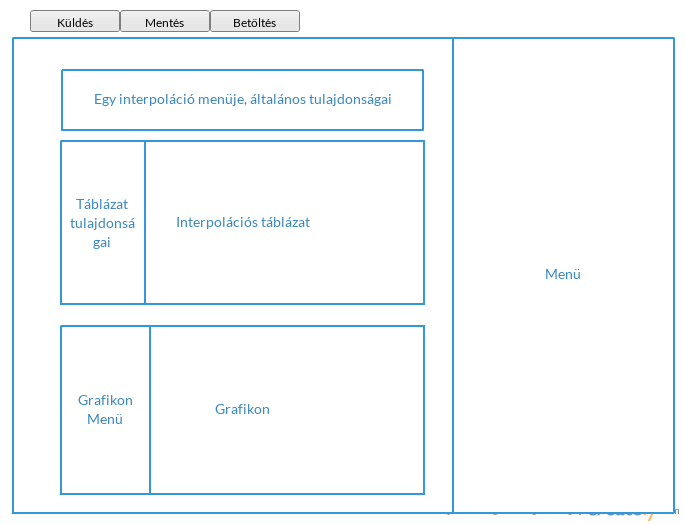
\includegraphics[width=\textwidth]{pics/weblap_vazlat}
\centering
\caption{Weboldal Vázlata}
\end{figure}

\begin{figure}[h]
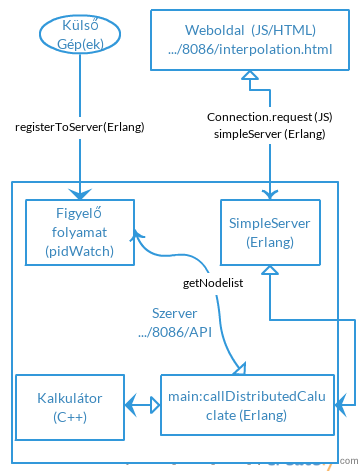
\includegraphics[width=8cm]{pics/kommunikacio}
\centering
\caption{Kommunikáció}
\end{figure}

\section{Weboldal}
Weboldal felépítése HTML és JavaScript segítségével valósult meg. Egy oldalból áll melyen a felhasználó össze állítja a neki szükséges adathalmazt. Új adathalmazokat hozhat létre, a régieket szerkesztheti. A háttérben JSON-be formálódnak az adatok.
Ha a felhasználó végzett egy gombra nyomással a program legenerálja a szükséges objektumot. \newline
A felület sok gombot tartalmaz, melyek hatására frissíthetőek az adatok. Amikor frissítünk egy részt, általában mentődnek az értékek egy inputba JSON formában.
\subsection{Felépítés}
	A weboldal forráskódja a Webpage mappában helyezkedik el. 
	A fájlszerkezet az alábbi:
	\begin{description}
		\item[webpage.js :] \hfill \\  Globális változók inicializálása és pár alapbeállítás lefuttatása
		\item[webpage.html :]  \hfill \\ Weboldal megjelenítése, fájlok betöltése
		\item[init] 
		\hfill \\ Inicializáló függvények hívásai és események
		\begin{description}
			\item[menulist.js : ] Interpolációk listájának inicializálója
		  	\item[plot.js : ] Interpolációs grafikon inicializálása
			\item[table.js : ] Interpolációs táblázat inicializálása
		 	\item[events.js : ] Gombra kattintások eseményei
		\end{description}

		\item[model] 
		\hfill \\ Objektumok, melyeket az inicializáló lépésben hívunk, és azok segédletei
		\begin{description}
		 	\item[base.js : ] Globális függvények
		 		\hfill \\ Base.get, Base.erlangJSON, Base.forEach
		 	\item[base\_table.js : ] Általános táblázat generáló függvény
		 	\item[connection.js : ] Szerver kapcsolat meghívására szolgáló függvény
		 		\hfill \\ Connection.request
		 	\item[plot\_types.js : ] A grafikon kirajzoló típus objektumai
		 	\item[polinome.js : ] Polinóm kirajzolását segítő függvények
		 		\hfill \\ makePolinome található benne és egyéb segédfüggvények
		 	\item[web\_page\_debug.js : ] A Weboldalon történő logolást segítő objektum
		 	\hfill \\ Jelenleg sehol nem használjuk már, de a megvalósítás során fontos szerepe volt a hibajavításban
		\end{description}
		\item[model/interpolation] 
		\hfill \\ Az oldal 3 fő részegységének függvényei
			\begin{description}
			\item[menulist.js : ] Interpolációk lista megvalósítása
			\hfill \\  function interpolationMenulist (aConfig) Objektum fájlja
		  	\item[plot.js : ] Interpolációs grafikon megvalósítása
			\hfill \\  function interpolationPlot(aConfig) Objektum fájlja
			\item[table.js : ] Interpolációs táblázat megvalósítása
			\hfill \\  function interpolationTable(aConfig) Objektum fájlja
			\end{description}
	\end{description}
\subsection{Fontsabb objektumok és függvények}
	\hfill
	Az objetumokat legtöbb esetben egy függvény generálja, melyben that.-al jelöltek azok, melyeket a visszatérés után felhasználunk az eseménykezelésekhez.
	\begin{description}
		\item[makePolinome(inPolinome, plotFor)] 
			\hfill \\ 
			Polinóm pontjainak legenerálására szolgáló függvény, a grafikon kirajzolónak megfelelő típusban
			\begin{description}
			\item[inPolinome] polinóm
			\item[plotFor] polinóm intervalluma és pontossága
			\end{description}
		\item[Connection.request(aConfig)] 
			\hfill \\ 
			Elküldi a szervernek az értékeket
			\begin{description}
			\item[aConfig.params] a kommunikáció objektuma
			\item[aConfig.callback] sikeres visszatérés esetén lefutó függvény
			\end{description}
		\item[basicTable (aConfig)]
			\hfill \\ 
			Egy alap tábla létrehozó objektum. Ennek segítségével tudtam létrehozni az interpolációs táblázatot és a menülistát(interpoláció választó)
			\begin{description}
			\item[that.addNewCellToRow(rowIndex, textValue, inputAttributes)] 
				\hfill \\  Ad egy új cellát a sorhoz
			\item[that.addNewRowToTable(data)]
				\hfill \\ Ad egy új sort a táblázathoz
			\item[that.addNewColumnToTable(data)]
				\hfill \\ Ad egy új oszlopot a táblázathoz
			\item[that.newTable()] 
				\hfill \\ Új tábla létrehozása
			\item[that.setCellForm((i , j, attributes))] 
				\hfill \\ Egy adott cella megformázás beállítása
			\item[that.getNumOfCols()] 
			 	\hfill \\ Vissza adja az oszlopok számát
			\item[that.getNumOfRows()]
				\hfill \\ Vissza adja a sorok számát
			\item[that.getRow(i)]
				\hfill \\ Vissza adja a sort az index alapján. 
				Ha nincs olyan indexű akkor null
			\item[that.getInputTag(i, j)]
				\hfill \\ Vissza tér a tábla input elemével
			\item[that.getValue(i, j)]
				\hfill \\ Egy adott cella érték lekérdezése
			\item[that.findValue(column, value)] 
				\hfill \\ Megkeresi melyik sorban van egy adott értéket
			\item[that.setValue(i, j, value, form)]
				\hfill \\ Beállít egy adott értéket egy cellának
			\item[that.deleteTable()]
				\hfill \\ Teljesen törli a táblázatot
			\item[that.remove(row)]
				\hfill \\ Kivesz egy sort a táblázatból
			\item[addNewRowTagToTable ()]
				\hfill \\ Ad egy új sort a táblázathoz
			\item[addCellToRow(index)]
				\hfill \\ Ad  egy cellát a sorhoz
			\item[setAttributes(object, attributes)]
				\hfill \\ Beállítja egy objektum tulajdonságait
			\item[makeTextInput (value,  attributes)]
				\hfill \\  TextInput hozzáadása a sorhoz
			\end{description}
		\item[interpolationMenulist (aConfig)] 
			\hfill \\ 
			Az interpolációs menü függvénye. Itt tarjuk számon az aktuálisan betöltött adathalmazt.
			\begin{description}
			\item[that.newItem()] 
			\hfill \\ Új Lista elem
			\item[that.getDataArray(server)] 
			\hfill \\ Vissza adja az adathalazt, tömb formában. Ebben a formában küldjük fel a szervernek.
			\item[that.getDataObject()] 
			\hfill \\ Vissza adja az adathalmazt, egy objektum formájában. Az Objektum értékeinek kulcsa, az interpolációk id-ja.
			\item[that.saveItemSettings()] 
			\hfill \\ Elmenti az adatokat az aktuálisan kijelölt sorba.
			\item[that.loadItemSettings(index)]
			\hfill \\ Feldogozza az adatt sort a táblából, és betölti az adatokat a táblába.
			\item[that.loadAll(savedObject, resultObject)] 
			\hfill \\Betölti az összes Interpolációt az adott adathalmazból
			\item[newMenulist()] 
			\hfill \\
			Új menülista: régi menü kitörlése, és egy új generálása
			\hfill \\ 
			\end{description}
		\item[interpolationPlot (aConfig)]
			\hfill \\ Grafikon megjelenítése: Flot segítségével létrehoztam az alábbi Objektumot. Ebben valósítottam meg a kirajzolást, és annak tulajdonságait.
			\begin{description}
			\item[that.refresh(points, polinomials)]
			\hfill \\ Pontok és a polinómok alapján frissíti a grafikont
			\item[that.getPlotSettings]
			\hfill \\ Visszatér a grafikon megjelenítési tulajdonságokkal. Ennek segítségével mentjük el a tulajdonságokat.
			\item[that.setPlotSettings]
			\hfill \\ Betölti a grafikon megjelenítési tulajdonságokat.
			\item[generateData(senderData, polynomial)]
			\hfill \\ Legenrálja a grafikon azon bemenő paraméterét, amely a megjelnítendő adatokat állítja
			\item[generateType()]
			\hfill \\ Legenrálja a grafikon azon bemenő paraméterét, amely a grafikon megjelítését állítja
			\item[setDefaultSettings()]
			\hfill \\ Legenrálja a grafikon azon bemenő paraméterét, amely a grafikon megjelítését állítja
			\item[generatePointSet(tableArray, derivNum)]
			\hfill \\ Legenerálja az adott pontokat, az interpolációs táblázatból
			\end{description}

		\item[interpolationTable (aConfig)]
			\hfill \\ 
				Az interpolációs Táblázat logikája, és generálása. Ebben a táblázatban tekinthetjük meg a pontokat.
			\begin{description}
			\item[that.addPoint(x, y, dn)] 
			\hfill \\ Hozzá adja a pontot a táblázathoz. Ha létetik ezen az X-en pont akkor frissíti.
			\item[that.setPoints(tableArray)] 
			\hfill \\ Feltölti a táblázatot egy adott tömb értékeivel
			\item[that.setData(data)] 
			\hfill \\ Feltölti az adatokkal a táblát
			\item[that.getData()] 
			\hfill \\ Vissza adja a táblázatban szereplő adatok
			\item[that.getPoints()] 
			\hfill \\ Vissza adja a táblázatban szereplő pontokat
			\end{description}
	\end{description}

\subsection{Kommunikáció}
\subsection{Tesztelési terv}

\section{Elosztott rendszer}
Elosztott rendszer Erlang-ban lett megvalósítva. Az elosztást interpolációnként végezzük, vagyis annyi node-ot hozunk létre amennyi interpolációt kívánunk egyszerre kiszámítani.
\subsection{Web-szerver kommunikáció}
\paragraph{Adat feldolgozás}
Az elosztott rendszer először kap egy JSON adathalmazt melyből kinyeri a neki szükséges adatokat, és átkonvertálja.
\subsection{Gép-szerver kommunikáció}
\subsection{Elosztás folyamata}
\subsection{Tesztelési terv}

\section{Kalkulátor}
A Kalkulátor részben számítódik ki egy-egy interpolációnak az ereménye.
A megkapott adatok alapján számol, ha kell létre hozza a kezdő mátrixot, kiszámolja az eredmény mátrixot, majd annak segítségével kiszámolja a polinómot.
\subsection{Fontosabb számítási függvények}

\begin{description}
	\item[DArray interpolateMain] 
	\hfill \\ Kívülről meghívandó fő függvény mely elosztja és konvertálja a részeket
	\begin{description}
	  \item[DArray \&x :] Az x pontok listája 
	  \item[DMatrix \&Y :] Az x pontokhoz tartozó y pontok halmaza
	  \item[string type :] Interpóláció típusa: lagrange, newton, hermite
	  \item[bool inverse :] Inverz interpoláció kell-e
	\end{description}
\end{description}
\subsection{Elosztott rendszerrel való kommunikáció}
Az elosztott rendszerben hívódó számítást Erlang - erl\_nif"-el sikerült megoldanom. 
Az ezzel kapcsolatos dolgokat az Calculator/erlang.cpp tartalmazza. 
\subsection{Tesztelési terv}
A tesztelést folyamatosan végeztem a minta adatok alapján. A függvények implementálása közben ezekre a minta adatokra meghívtam, majd ezekkel számoltam. A teszteléshez a logTest.cpp fájlban található függvényeket alkalmaztam. 


\begin{thebibliography}{9}
\bibitem{numanalbev}
Gergó Lajos: Numerikus Módszerek, ELTE EÖTVÖS KIADÓ, 2010, [329], ISBN 978 963 312 034 7
\bibitem{} {http://www.erlang.org/doc/man/erl\_nif.html} 2015
\bibitem{} {https://www.sharelatex.com/learn/Sections\_and\_chapters} 
2015
\bibitem{} {https://github.com/mochi/mochiweb/blob/master/src/mochijson.erl} 2015
\bibitem{} {http://tex.stackexchange.com/questions/137055/lstlisting-syntax-highlighting-for-c-like-in-editor} 2015
\end{thebibliography}

\end{document}
